\begin{figure*}
  \centering
  \subfigure[No wear leveling]{\label{fig::WearLeveling::None} 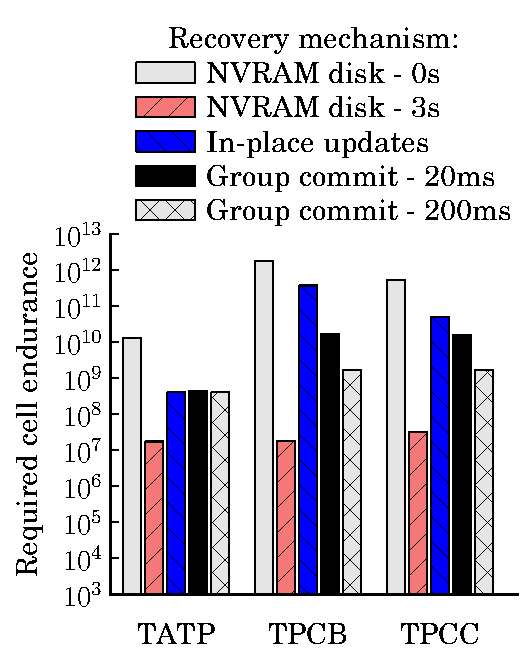
\includegraphics[width=.45\textwidth]{OLTP_eval/WearLeveling_None.pdf}}
  \subfigure[Perfect wear leveling]{\label{fig::WearLeveling::Perfect}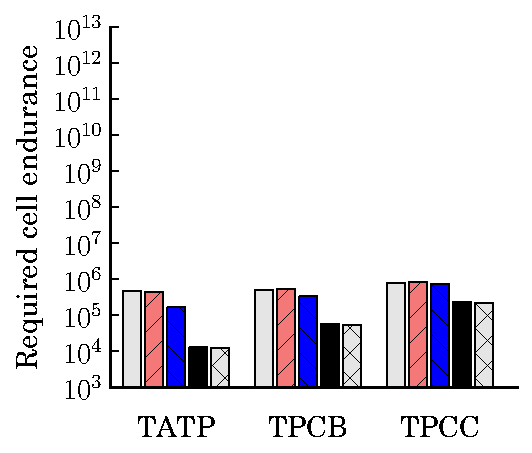
\includegraphics[width=.45\textwidth]{OLTP_eval/WearLeveling_Perfect.pdf}}
  \caption{\textbf{NVRAM cell endurance for 10-year lifetime.}  Without hardware wear leveling the most-written cell limits device lifetime.  \NVDisk requires conservative page flushing (3s recovery latency vs 0s, instantaneous, recovery) and \GroupCommit requires longer batch periods (200ms vs 20ms) to improve device lifetime.  We expect hardware wear leveling to always be required with \InPlace.  With perfect wear leveling (all writes occur evenly throughout cells in the device) and a 32GB storage device all workloads and configurations achieve a 10-year device lifetime for cell endurance of $10^6$ writes and greater.}
  \label{fig::WearLeveling}
\end{figure*}
